\chapter{\IfLanguageName{dutch}{Stand van zaken}{State of the art}}
\label{ch:stand-van-zaken}

% Tip: Begin elk hoofdstuk met een paragraaf inleiding die beschrijft hoe
% dit hoofdstuk past binnen het geheel van de bachelorproef. Geef in het
% bijzonder aan wat de link is met het vorige en volgende hoofdstuk.

% Pas na deze inleidende paragraaf komt de eerste sectiehoofding.
In deze stand van zaken worden de gebruikte technologieën stapsgewijs besproken om het nodige inzicht te creëren in het onderwerp chaos engineering. Eerst zal uitgelegd worden wat virtualisatie is en welke voordelen dit met zich meebrengt.
Vervolgens komt containervirtualisatie aan bod, en wat deze technologie teweeg heeft gebracht in de denkwijze rond softwarearchitectuur. Nadien zal uitleg gegeven worden over wat containerorchestratie is, hoe het er voor zorgt dat applicaties dynamisch kunnen schalen en hoe er gemikt wordt naar een zo hoog mogelijke uptime ervan. Tot slot wordt besproken wat chaos engineering inhoudt en wat de link is met containerorchestratie.   

\section{Virtualisatie}

Virtualisatie maakt het mogelijk om op een fysieke computer meerdere virtuele machines uit te voeren, elk met zijn eigen besturingssysteem, geheugen, processorkernen en opslagcapaciteit.

Het essentiële onderdeel om de virtuele machines te binden aan de hardware van de fysieke host, en wat de dynamische toewijzing van resources zoals geheugen en CPU mogelijk maakt, is een softwarelaag die men de hypervisor noemt. 

\subsection{Voordelen van een hypervisor}

Het gebruik van een hypervisor om virtuele machines op een host aan te maken heeft enkele voordelen:
\begin{itemize}
    \item Snelheid: virtuele machines opzetten verloopt snel i.v.m. een fysieke server opzetten.
    \item (Kost)efficiëntie: men maakt optimaal gebruik van de beschikbare resources op de host door deze dynamisch te verdelen over meerdere virtuele machines.   
    \item Overdraagbaarheid: virtuele machines worden bewaard als bestanden op de host en zijn makkelijk overdraagbaar naar andere systemen.
\end{itemize}

\subsection{Types hypervisors}

Er bestaan twee hypervisor types:
\begin{itemize}
    \item Type 1: bare-metal / native
    \item Type 2: hosted
\end{itemize}

Een bare-metal of native type 1 hypervisor is virtualisatiesoftware die rechtstreeks geïmplementeerd is op de hardware van een host en zich gedraagt zoals een lichtgewicht besturingssysteem. Het voordeel bij dit type hypervisor is dat geen volwaardig besturingssysteem geïnstalleerd wordt en dat het hiermee gevrijwaard blijft van de kwetsbaarheden die dit met zich meebrengt. Voorbeelden van type 1 hypervisors zijn VMware ESXi, Microsoft Hyper-V, Citrix Xen ... 

Een hosted type 2 hypervisor is software die bovenop het bestaande besturingssysteem op een host aanwezig is. Het nadeel bij een type 2 hypervisor is de verhoogde latentie doordat de communicatie tussen hardware en hypervisor eerst nog het besturingsssysteem moet passeren. Bekende voorbeelden hiervan zijn de softwarepakketten VirtualBox of VMware.

\begin{figure}[h]
    \centering
    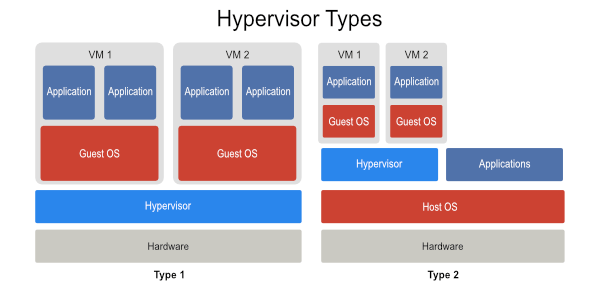
\includegraphics[scale=.7]{img/Hypervisor-Types.png}
    \caption{hypervisor types \autocite{Vembu2019}}
    \label{fig}
\end{figure}


\section{Containerisatie}

Klassieke softwareontwikkeling leverde applicaties op die gebaseerd waren op een monolitische architectuur. Hierin was alle code aanwezig van de applicatie, zowel front- als backend. 
In moderne softwareontwikkeling maakt men gebruik van een microservices architectuur. Deze manier van softwareontwikkelling splitst de applicatie op in verschillende services, die elk hun eigen code bevatten.

Het grootste voordeel van deze manier van softwareontwikkeling is de flexibiliteit om de applicatie aan te passen.  

\begin{figure}[h]
    \centering
    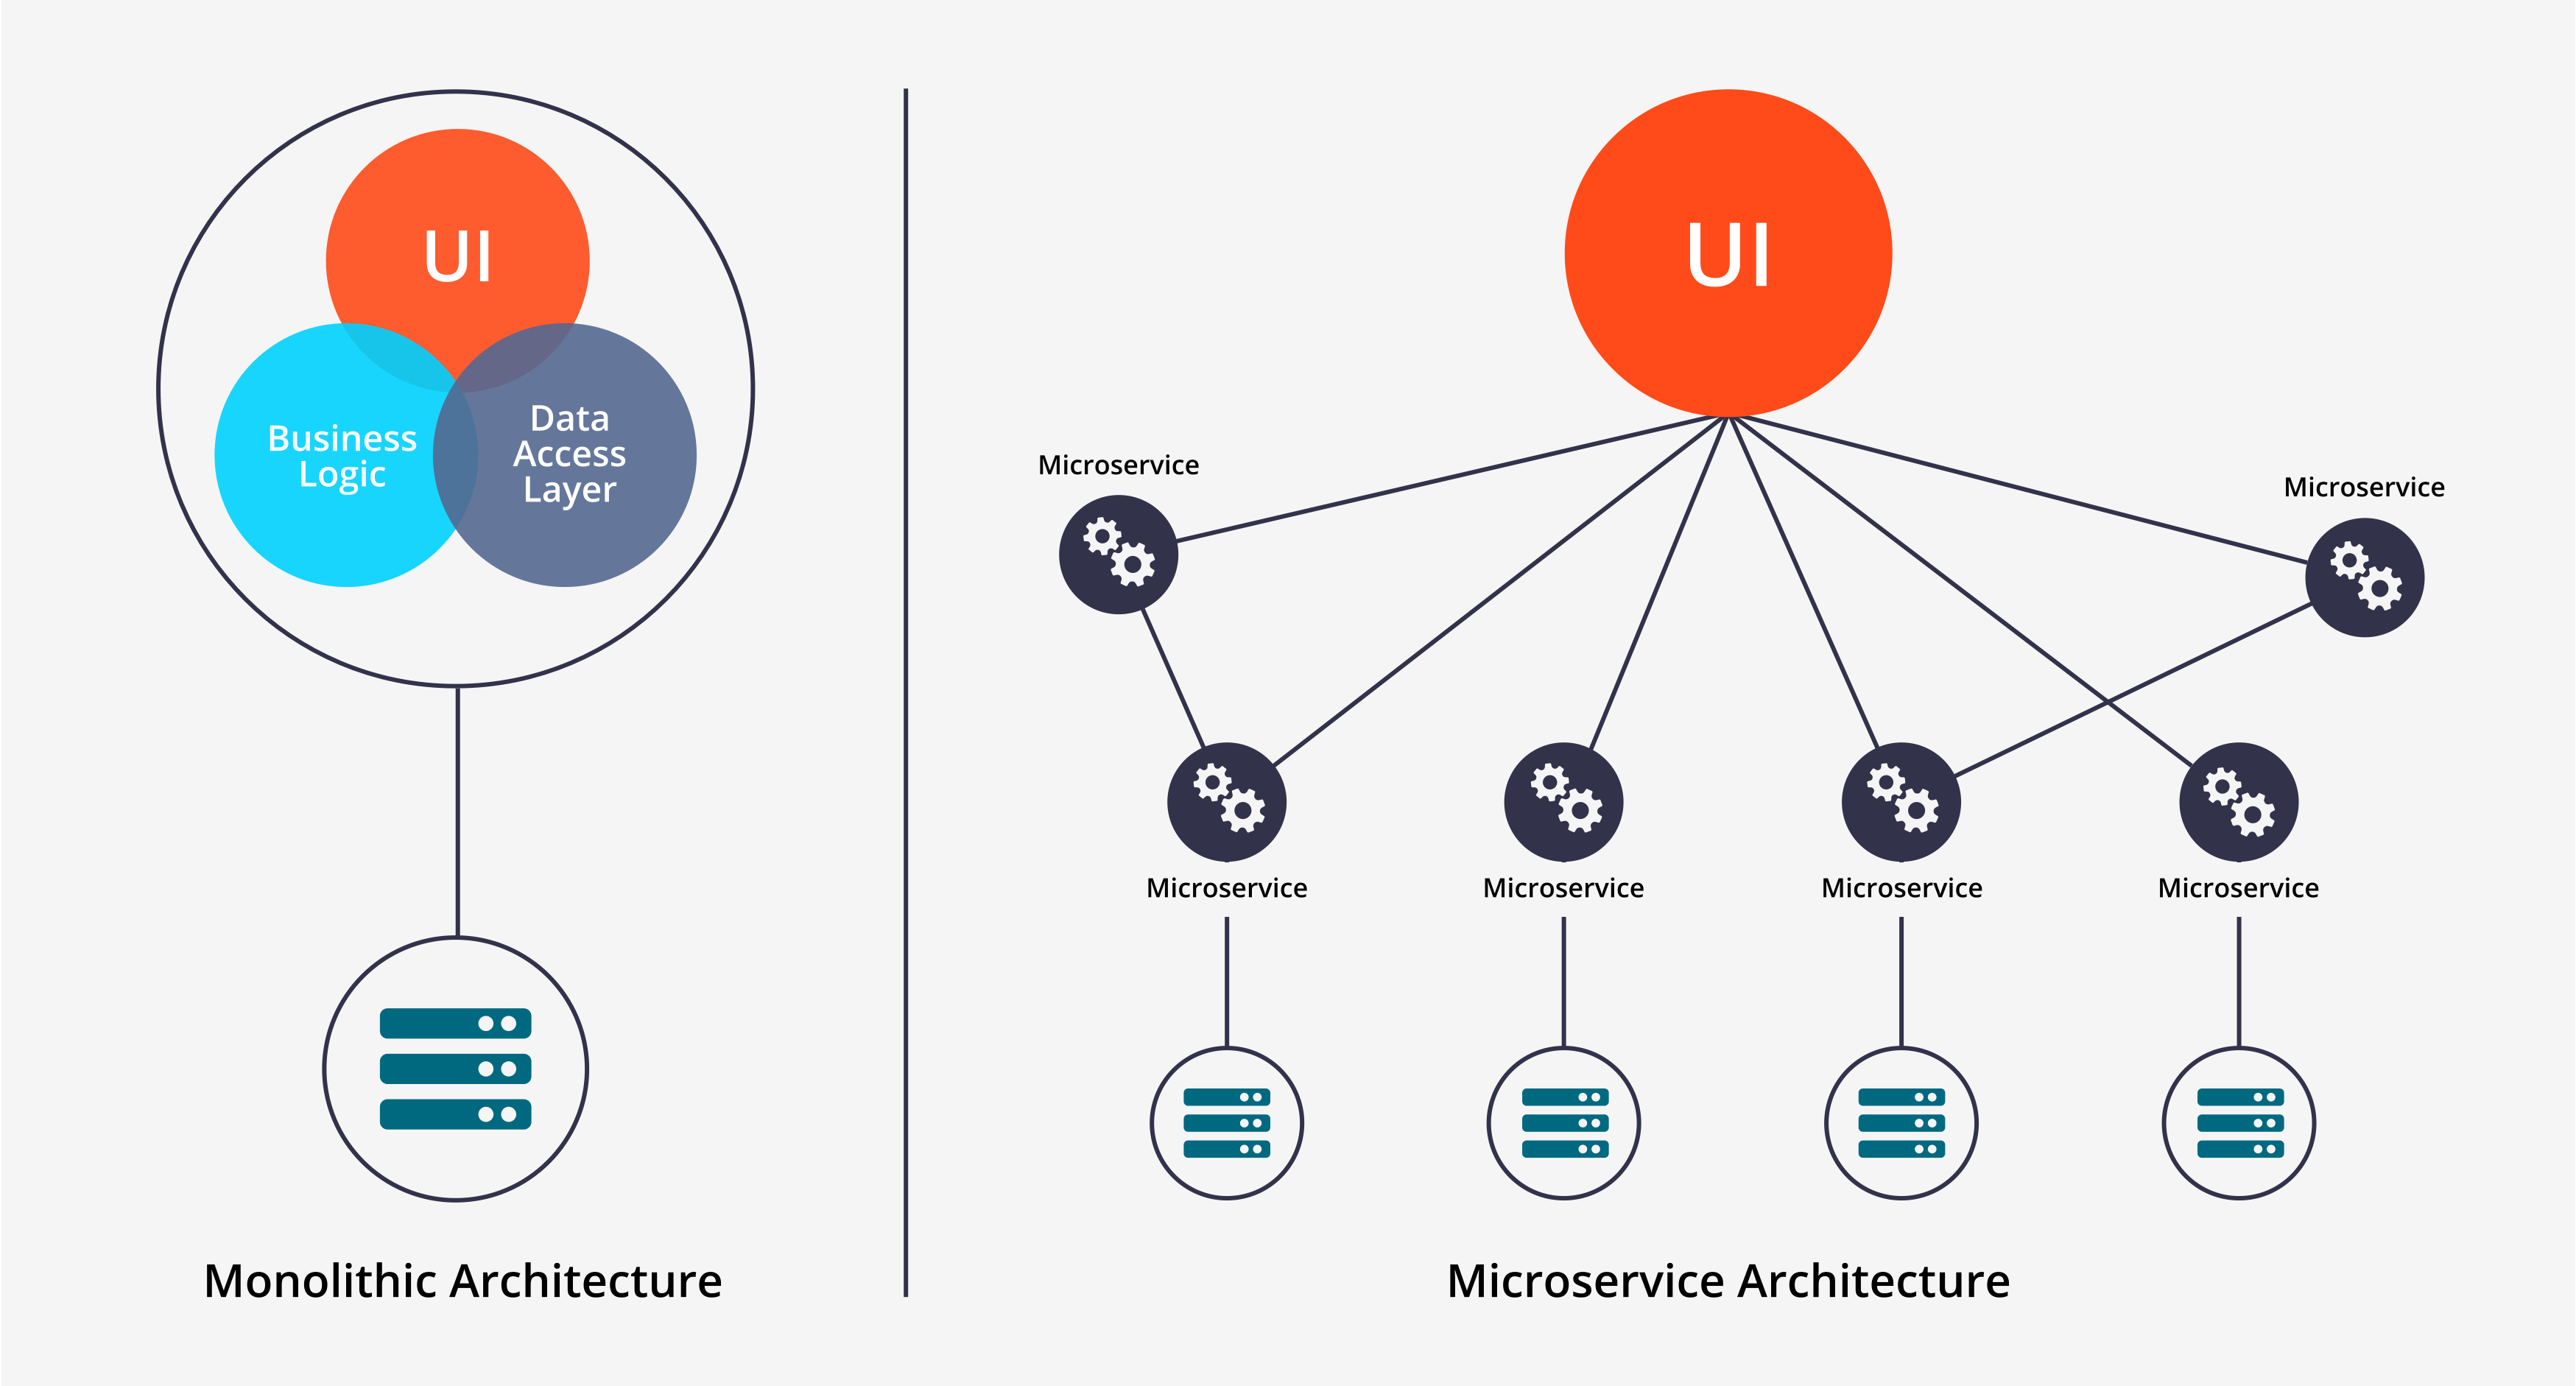
\includegraphics[scale=.1]{img/monolithic_vs_microservices.png}
    \caption{hypervisor types \autocite{Sanjaya2020}}
    \label{fig}
\end{figure}

Services van zulke moderne applicaties worden ondergebracht in containers. Een container op zich bevat geen besturingssysteem maar verpakt en isoleert de code van één applicatie inclusief de gerelateerde configuratiebestanden en afhankelijkheden die deze nodig heeft. Het voordeel van containers is dat ze snel opgestart kunnen worden doordat ze weinig resources vereisen, en makkelijk overdraagbaar zijn naar verschillende omgevingen. Meerdere containers kunnen actief zijn op een systeem en maken ook allemaal gebruik van hetzelfde besturingssysteem. \autocite{Singh2020}

Ondanks dat containers net zoals virtuele machines een vorm van virtualisatie zijn, is er toch een belangrijk onderscheid te maken. Containers zijn namelijk een vorm van besturingssysteemvirtualisatie, dit tegenover virtuele machines die aan hardwarevirtualisatie doen.
Hierdoor verbruiken containers dus minder resources ten opzichte van virtuele machines. \autocite{Holt2018}

Containers blijven wel afhankelijk van het besturingssysteem. Men kan geen Windows containers in een Linux omgeving opstarten of omgekeerd. Om de interactie met het besturingssysteem op de host mogelijk te maken is een container engine op het systeem nodig zoals Docker, CRI-O, LXC ... 

Een container heeft een image nodig.   

Containers en virtuele machines kunnen gecombineerd worden om virtuele omgevingen te maken waarin software ontwikkeld en getest kan worden.

\section{Containerorchestratie}

\section{Chaos Engineering}
  
Dit hoofdstuk bevat je literatuurstudie. De inhoud gaat verder op de inleiding, maar zal het onderwerp van de bachelorproef *diepgaand* uitspitten. De bedoeling is dat de lezer na lezing van dit hoofdstuk helemaal op de hoogte is van de huidige stand van zaken (state-of-the-art) in het onderzoeksdomein. Iemand die niet vertrouwd is met het onderwerp, weet nu voldoende om de rest van het verhaal te kunnen volgen, zonder dat die er nog andere informatie moet over opzoeken \autocite{Pollefliet2011}.

Je verwijst bij elke bewering die je doet, vakterm die je introduceert, enz. naar je bronnen. In \LaTeX{} kan dat met het commando \texttt{$\backslash${textcite\{\}}} of \texttt{$\backslash${autocite\{\}}}. Als argument van het commando geef je de ``sleutel'' van een ``record'' in een bibliografische databank in het Bib\LaTeX{}-formaat (een tekstbestand). Als je expliciet naar de auteur verwijst in de zin, gebruik je \texttt{$\backslash${}textcite\{\}}.
Soms wil je de auteur niet expliciet vernoemen, dan gebruik je \texttt{$\backslash${}autocite\{\}}. In de volgende paragraaf een voorbeeld van elk.

\textcite{Knuth1998} schreef een van de standaardwerken over sorteer- en zoekalgoritmen. Experten zijn het erover eens dat cloud computing een interessante opportuniteit vormen, zowel voor gebruikers als voor dienstverleners op vlak van informatietechnologie~\autocite{Creeger2009}.

\lipsum[7-20]
